% LaTeX template for Lab Reports
% Copyright (C) 2014 Julian Coy

%% CHANGE REPORT TITLE HERE
\newcommand{\reporttitle}{
 Simple Processor
}

%% HEADER/PREAMBLE INFORMATION

% "The font should be 11pt Times New Roman"
\documentclass[11pt]{report}
\usepackage[T1]{fontenc}
\usepackage[utf8]{inputenc}

\usepackage{mathptmx}               

% "The body of the paper should use 1" margins on all sides."
\usepackage[margin=1in]{geometry}

% "Pages must be numbered, starting with 1 on the first page in the body of the report.
% The cover page should not be numbered. 
% Page numbers should be in the bottom-right corner of the page."
\usepackage{fancyhdr}
\pagestyle{fancy}
\fancyhead{}
\fancyfoot{}
\renewcommand{\headrulewidth}{0pt}
\fancyfoot[R]{\thepage}

% Set up customized spacing
\usepackage{setspace}

% Allows for Trademark Symbols
\usepackage{textcomp}

% Remove spacing between items in lists
\usepackage{enumitem}

% Remove extra spacing between titles of sections and subsections
\usepackage{titlesec}
\titlespacing\section{0pt}{10pt}{10pt}
\titlespacing\subsection{0pt}{10pt}{10pt}
\titlespacing\subsubsection{0pt}{0pt plus 4pt minus 2pt}{0pt plus 2pt minus 2pt}

% Setup the specialized chapter section for the Abstract
\titlespacing\chapter{0pt}{0pt plus 4pt minus 2pt}{0pt plus 2pt minus 2pt}
\titleformat{\chapter}[block]{\centering\Huge}{}{}{}{}

% Set up BibTeX integration using IEEE citation format
\usepackage{cite}
\bibliographystyle{ieeetr}
\usepackage{url}

% Set bibliography to have a section header rather than chapter header
\makeatletter
\renewenvironment{thebibliography}[1]
     {\section*{\scshape Works Cited}% <-- this line was changed from \chapter* to \section*
      \@mkboth{\MakeUppercase\bibname}{\MakeUppercase\bibname}%
      \list{\@biblabel{\@arabic\c@enumiv}}%
           {\settowidth\labelwidth{\@biblabel{#1}}%
            \leftmargin\labelwidth
            \advance\leftmargin\labelsep
            \@openbib@code
            \usecounter{enumiv}%
            \let\p@enumiv\@empty
            \renewcommand\theenumiv{\@arabic\c@enumiv}}%
      \sloppy
      \clubpenalty4000
      \@clubpenalty \clubpenalty
      \widowpenalty4000%
      \sfcode`\.\@m}
     {\def\@noitemerr
       {\@latex@warning{Empty `thebibliography' environment}}%
      \endlist}
\makeatother

% Set up math
\usepackage{amsmath}
\usepackage{amsfonts}
\usepackage{amssymb}

% Set up graphics
\usepackage{graphicx}
\usepackage{float}

% Set up tables
\usepackage{tabularx}
\usepackage{booktabs}

% Set up code blocks
% or not...

\usepackage{listings}
\usepackage{color}

\definecolor{dkgreen}{rgb}{0,0.6,0}
\definecolor{gray}{rgb}{0.5,0.5,0.5}
\definecolor{mauve}{rgb}{0.58,0,0.82}

\lstset{frame=tb,
  language=VHDL,
  aboveskip=3mm,
  belowskip=3mm,
  showstringspaces=false,
  columns=flexible,
  basicstyle={\small\ttfamily},
  numbers=none,
  numberstyle=\tiny\color{gray},
  keywordstyle=\color{blue},
  commentstyle=\color{dkgreen},
  stringstyle=\color{mauve},
  breaklines=true,
  breakatwhitespace=true
  tabsize=3
}

%% START OF DOCUMENT

\begin{document}

% "The main body of text should use 1.5 spacing"
\begin{spacing}{1.5}

% Suppress page numbering on first page
\thispagestyle{empty}

\begin{scshape}

% Title
% "The title should be centered and written in approximately 22pt font."
\vspace*{30pt}
{
\Huge
\begin{center}
    \reporttitle
\end{center}
}
\vspace{30pt}

% Team Number
% "The Team number should be centered and written several lines below the title and should use a
% similar size font as the title."
{
\Large
\begin{center}
  Lab Report 5 for ECE327 \\
  Digital Systems Design
\end{center}
}
\vspace{30pt}
% Team Members
% "Directly below the team identifier, team members should be listed alphabetically by last name, one
% per line, in approximately 14pt font. The column of names should be approximately centered on
% the page, but the names within the column should be left justified (so they all start at the same
% horizontal position)."
{
\Large 
\begin{center}
  Submitted by \\
  Julian Coy
\end{center}
}
\vspace{120pt}

{
\Large
\begin{center}
  Undergraduate of Electrical \& Computer Engineering \\
  Clemson University
\end{center}
}
\vspace{30pt}

{
\Large
\begin{center}
  April 28, 2014
\end{center}
}

\end{scshape}

% New page and reset page numbering
\clearpage

%% START EDITS BELOW %%

\vspace{15pt}
  \setcounter{chapter}{1}
  \chapter*{Abstract}
  \label{cha:abstract}
\vspace{72pt}

A system that can perform different operations based on numerical operations considered a processor.  Processors are the basic control units of all computing.  The task of this lab was to implement a simple processor system.  The first part of the lab was to build a processor that contained a full adder that was also capable of subtraction.  Located in the processor were 8 16-bit registers, as well as other registers required by the system (in this lab, two were needed).  The second part of the lab was to create a memory module that would feed the processor instructions by reading them sequentially from a ROM module.  The final portion of the lab was to identify critical paths in the processor circuit and then postulate methods to obtain the maximum viable frequency.

\vspace{4.5in}

\textit{Note: All clocks generated for simulation were built using Morten Zilmers clock gen package \cite{Synth}.}

\thispagestyle{empty} % clear page number
\clearpage
\setcounter{page}{1}

\section*{\scshape Introduction} %(0.5 pages)
\label{cha:introduction}

The purpose of this lab is to simulate a simple 16-bit processor.  A diagram of the system can be seen in Figure \ref{fig:system}.  The full adder/subtracter and multiplexer will operate instantaneously and not need to be operated by a clock.  The code for each module is provided in the code appendices at the end of the report.

\vspace{15px}
\begin{figure}[H]
    \centering
    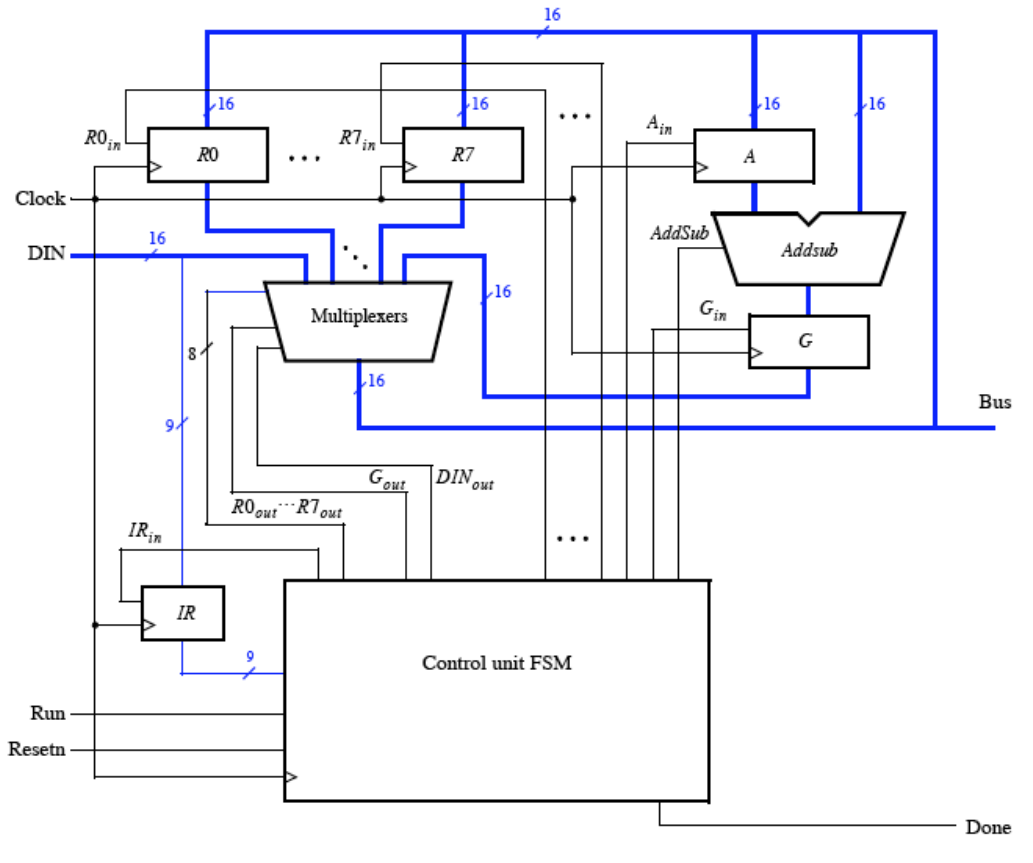
\includegraphics[width=1.0\textwidth,keepaspectratio]{system.png}
    \caption{Simple Processor}
    \label{fig:system}
\end{figure}

There are four main components to this design: the control state module, the registers, the multiplexer, and the full adder/subtracter.  The IR register is similar to the other registers, but only stores a 9 bit value.  The multiplexer logic is contained inside the control FSM due to it's simplicity.

\clearpage

\section{\scshape Lab 4 System Design} %(0.5 pages)
\label{sec:fsm_design}

\subsection{\scshape Register Design}
\label{sub:design_piso}

There are only two register prototypes in this design, and both are incredibly similar.  Registers 0-7, A, and G are all 16 bit flip flops.  They store a value on the rising edge of the clock only when their select line is driven high.  The instruction register (IR) is the exact same as the others, but only utilizes 9 bit buses and storage.

The only real variation in the registers is their data line connections.  Registers 0-7 feed from a 16 bit data bus and output to the multiplexer.  Register A feeds from the data bus as well, but instead of the multiplexer, it outputs to the full adder/subtracter (adder).  Register G's input is from the output of the adder unit and outputs back into the multiplexer.  The most different of the connections is again for the IR.  The IR captures the 9 MSBs of the data in (DIN) line.  It also outputs its data directly to the control unit.

\subsection{\scshape Testing of the Registers}
\label{sub:test_piso}

Due to the simplicity of the registers, only one unit test was required.  Figure \ref

\vspace{15px}
\begin{figure}[H]
    \centering
    \includegraphics[width=1.0\textwidth,keepaspectratio]{.png}
    \caption{Register A Results}
    \label{fig:rega}
\end{figure}

The test shown in Figure \ref{fig:rega} shows the manipulations that are performed on the multiplicand via register A.  Notice that as the load value goes high, the first code is produced: 100.  This code, and the following codes shown, align perfectly with the expectations for a bit-pair coding scheme.

\subsection{\scshape Testing of Registers B and D}
\label{sub:test_counter}

Registers B and D were tested at the same time to show that the counter will stop when the maximum number of shifts have occurred.  This was not necessary to do, but it aids the user in understanding why the counter is needed, as the controller has no other way of keeping track of the amount of shifts performed.

% \vspace{15px}
% \begin{figure}[H]
%     \centering
%     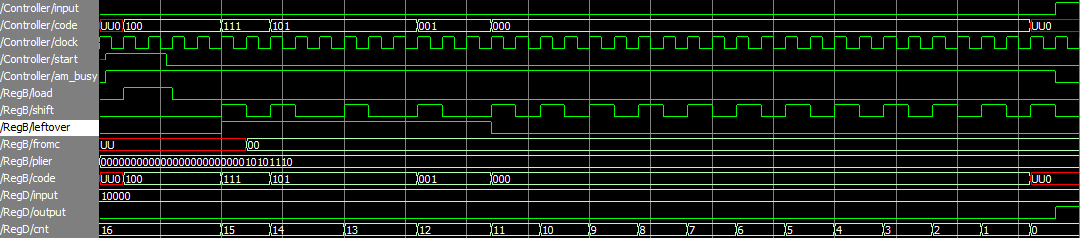
\includegraphics[width=1.0\textwidth,height=4cm,keepaspectratio]{reg_d_b.png}
%     \caption{Register D and B Test}
%     \label{fig:regd_b}
% \end{figure}

Notice that the shifts are spaced slightly.  This occurs when an add operation is warranted.  Later on in the register C test, you will be able to see the add signal being used.  The disparity between clock cycles used per operation is the reason for the counter.  Without it there would be know way to know preemptively how many clock cycles would be needed for a given multiplication.

\subsection{\scshape Testing of Register C}
\label{sub:design_fsm}

Register C was fairly simple to implement, once the other units were designed.  In the test, you will notice that the registers values change based upon the signal changes that occur upon the signals shift, add, and load.  Register C performed the same operations as B except it did not send off the lowest three bytes for coding purposes.

% \vspace{15px}
% \begin{figure}[H]
%     \centering
%     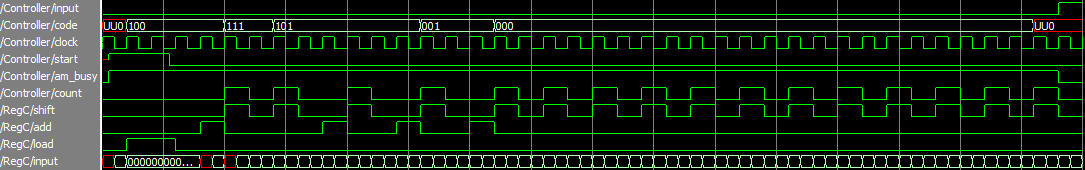
\includegraphics[width=1.0\textwidth,keepaspectratio]{reg_c.png}
%     \caption{FSM State Diagram}
%     \label{fig:diag_fsm}
% \end{figure}

\clearpage

\section{\scshape Conclusions} % (fold)
\label{sec:conclusions}

There are definite changes that could be made to this project to increase the efficiency and decrease the overall runtime of the algorithm.  Mainly making the system asynchronous.  Do do that, more signals would need to be added to the control unit.  In particular, bus read signals would be needed to make sure register C doesn't stomp out its own value through the adder loop.

Overall, this lab shows that complex algorithms can be implemented in VHDL by creating small modules, one piece at a time.  If anything else can be taken away, it is that testing is best done on INDIVIDUAL units, not groups.  By testing entities individually, debugging is greatly simplified and overall development time and stress are reduced.

% section scshape_conclusions (end)

% Bibliography

\bibliography{citationsfile}{}

\clearpage

\chapter*{\scshape Appendix A: Lab 4 Code}
\label{app:a}

\vspace{15px}
\begin{lstlisting}
-- something
\end{lstlisting}
\clearpage
\vspace{15px}
\begin{lstlisting}
-- something
\end{lstlisting}
\clearpage
\vspace{15px}
\begin{lstlisting}
-- something
\end{lstlisting}
\clearpage
\vspace{15px}
\begin{lstlisting}
-- something
\end{lstlisting}
\clearpage
\vspace{15px}
\begin{lstlisting}
-- something
\end{lstlisting}
\clearpage
\vspace{15px}
\begin{lstlisting}
-- something
\end{lstlisting}
\clearpage
\vspace{15px}
\begin{lstlisting}
-- something
\end{lstlisting}
\clearpage
\vspace{15px}
\begin{lstlisting}
-- something
\end{lstlisting}

%% END EDITS HERE %%

\end{spacing}

\end{document}

%%%%%%%%%%%% Extra stuff for use later

% \begin{itemize}[noitemsep,nolistsep]
%     \item \emph{Choose off-the-shelf parts} rather than self-made parts whenever possible.
%     \item \emph{Reuse and expand on open-source software libraries} to avoid spending time writing code that duplicates functionality that already exists elsewhere (and is likely more robust).
%     \item \emph{Keep the hardware simple} by using the least amount of hardware necessary for operation to avoid additional potential points of failure.
%     \item \emph{Modularize systems and components}. Each component should do one thing and do it well.
% \end{itemize}
% Figure \ref{BlockDiagram} shows a block diagram of the subsystems used in our design.

% \begin{figure}[H]
%     \centering
%     \caption{Block Diagram of Subsystems}
%     \label{BlockDiagram}
% \end{figure}
%     {
%     \centering
%       \includegraphics[width=\textwidth]{CostAccounting}
%     }